\documentclass[a4paper,10pt,oneside]{article}
\usepackage[polutonikogreek,italian]{babel}
\usepackage[utf8x]{inputenc}
\usepackage{amsmath}
\usepackage{amsthm}
\usepackage{amssymb}
\usepackage{amscd}
\usepackage{graphicx}
\usepackage{float}
\usepackage{array}
\usepackage{rotating}
\usepackage[small]{caption}
\usepackage{lscape}
\usepackage{fancybox}
\usepackage{booktabs}
\usepackage[noanswer]{exercise}
\parindent0ex
\renewcommand{\fboxsep}{0.4cm}
\usepackage{hyperref}
\renewcommand{\textfraction}{0.05}
\renewcommand{\topfraction}{0.95}
\renewcommand{\bottomfraction}{0.95}
\renewcommand{\floatpagefraction}{0.35}
\renewcommand{\ExerciseName}{Esercizio}
\renewcommand{\ExerciseListName}{Es}
\setcounter{totalnumber}{5}
\restylefloat{figure}
\begin{document}
\section*{Il pendolo semplice}


Il pendolo semplice è costituito da una massa puntiforme $M$ fissata all'estremità inferiore di un'asticella di massa trascurabile e lunghezza $L$, il sistema è libero di ruotare attorno all'estremità superiore dell'asta. Applichiamo la seconda legge di Newton alla massa sospesa, scomponiamo la forza di gravità lungo due direzioni: una perpendicolare all'asticella, l'altra parallela. Notiamo subito che siccome la massa è vincolata,  essa non si potrà muovere nella direzione radiale: la componente della forza in tale direzione non produrrà quindi alcun moto. Il termine significativo (della forza di gravità)  sarà quindi unicamente quello perpendicolare all'asticella.
La componente perpendicolare  si può ottenere con un po' di trigonometria:
\begin{equation}\label{pendolo_completo}
 F=-mg\sin\theta
\end{equation}
dove $\theta$ è l'angolo formato con la verticale figura [\ref{fig:pendolo_semplice}].
\begin{figure}[H]
 \centering
 \includegraphics[width=0.8\textwidth]{./immagini/pendolo_semplice.png}
 % pendolo_semplice.png: 2059x2444 pixel, 250dpi, 20.92x24.83 cm, bb=0 0 593 704
 \caption{Il pendolo semplice di lunghezza $L$ e massa $M$}\label{fig:pendolo_semplice}
\end{figure}
L'equazione [\ref{pendolo_completo}] non è risolubile per vie elementari. Fortunatamente è possibile introdurre un'approssimazione in grado di trasformare l'equazione [\ref{pendolo_completo}] in una forma a noi nota. Ricordando quanto detto nel calcolo dell'accelerazione centripeta nel moto circolare uniforme, possiamo approssimare il seno di un angolo con la sua ampiezza in radianti, se l'angolo è piccolo\footnote{È possibile calcolare che se vale la relazione $|\theta|<0.1$ l'errore è sufficientemente piccolo per poter applicare l'approssimazione nella gran parte dei casi.}
\begin{equation}
 \sin\theta\simeq \theta\quad \theta\to 0
\end{equation}
utilizzando questa approssimazione possiamo riscrivere la [\ref{pendolo_completo}] come:
\begin{equation}
 F=-mg\theta
\end{equation}
o introducendo la lunghezza dell'asta del pendolo:
\begin{equation}\label{pendolo_semplice}
 F=-\frac{mg}{L}L\theta
\end{equation}
dove il prodotto $L\theta$ rappresenta lo spostamento $x$, lungo l'asse delle ascisse, della massa collegata al pendolo. Questo  ci permette di riscrivere l'equazione [\ref{pendolo_semplice}] come:
\begin{equation}\label{pendolo_semplice_2}
 F=-\frac{mg}{L}x
\end{equation}
 se ora confrontiamo la [\ref{pendolo_semplice_2}] con l'equazione della forza per la massa in moto circolare uniforme:
\begin{equation}
 F_x=-m\omega^2x
\end{equation}
 vediamo che se le costanti che moltiplicano lo spostamento $x$ sono uguali allora i due moti risulteranno indistinguibili:
\begin{equation}
 \frac{mg}{L}=m\omega^2
\end{equation}
da cui si può vedere che il valore di $\omega$ deve essere:
\begin{equation}
 \omega=\sqrt{\frac g L}
\end{equation}
e il periodo del pendolo:
\begin{equation}
 T=2\pi\sqrt{\frac L g}
\end{equation}
Per il calcolo dell'energia potenziale del pendolo notiamo che, quando l'asticella forma un angolo $\theta$ con la verticale, il pendolo si trova alla quota $L(1-\cos\theta)$ come si può intuire dalla figura [\ref{fig:pendolo_semplice}]. Siccome il campo gravitazionale è conservativo il lavoro che questo compie durante lo spostamento della massa è indipendente dal percorso, la variazione di energia potenziale gravitazione dell'equipaggio del pendolo è quindi dipendente unicamente dalla quota  a cui si trova, ricordando che l'energia potenziale gravitazionale è:
\begin{equation}
 U=mgh
\end{equation}
possiamo scrivere
\begin{equation}
 U=mgL(1-\cos\theta)
\end{equation}
che nel caso di piccole oscillazione ovvero di moto armonico del pendolo diventa:
\begin{equation}
 U=\frac{1}{2}mgL\theta^2
\end{equation}
che ricorda fortemente l'energia potenziale elastica.


\end{document}
